\section*{The Problem of Overfitting}
Consider the problem of predicting y from $x \in R$. The leftmost figure \ref{fig:w3_overfit} shows the result of fitting a $y=\theta_0 + \theta_1 x$ to a dataset. We see that the data doesn't really lie on straight line, and so the fit is not very good.
\begin{figure}[ht]
\center
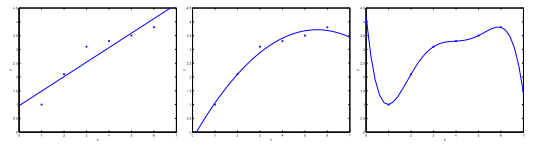
\includegraphics[scale=0.7]{W3_overfitting}
\caption{The Problem of Overfitting}
\label{fig:w3_overfit}
\end{figure}

Instead, if we had added an extra feature $x^2$, and fit $y = \theta_0 + \theta_1x + \theta_2x^2$, then we obtain a slightly better fit to the data (See middle figure). Naively, it might seem that the more features we add, the better. However, there is also a danger in adding too many features: The rightmost figure is the result of fitting a $5^{th}$ order polynomial $y = \sum_{j=0} ^5 \theta_j$. We see that even though the fitted curve passes through the data perfectly, we would not expect this to be a very good predictor of, say, housing prices (y) for different living areas (x). Without formally defining what these terms mean, we'll say the figure on the left shows an instance of {\bf underfitting}-in which the data clearly shows structure not captured by the model-and the figure on the right is an example of {\bf overfitting}.

Underfitting, or high bias, is when the form of our hypothesis function h maps poorly to the trend of the data. It is usually caused by a function that is too simple or uses too few features. At the other extreme, overfitting, or high variance, is caused by a hypothesis function that fits the available data but does not generalize well to predict new data. It is usually caused by a complicated function that creates a lot of unnecessary curves and angles unrelated to the data.

This terminology is applied to both linear and logistic regression. There are two main options to address the issue of overfitting:
\begin{itemize}
	\item[$1)$] Reduce the number of features:
	\item	\quad Manually select which features to keep.
	\item	\quad Use a model selection algorithm (studied later in the course).
	\item[$2)$] Regularization
	\item	\quad Keep all the features, but reduce the magnitude of parameters $\theta_j$
	\item	\quad Regularization works well when we have a lot of slightly useful features.
\end{itemize}